%----------------------------------------------------------------------------------------
%	SLIDE 3.
%----------------------------------------------------------------------------------------
\begin{frame}
\frametitle{Linux? Unix? GNU? OS???}


\only<1,6>{
\begin{figure}
	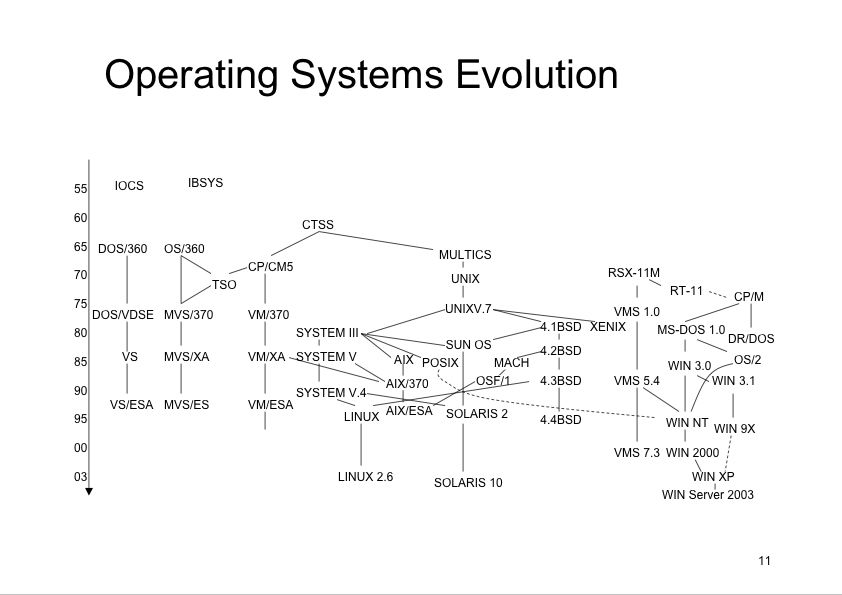
\includegraphics[width=0.85\textwidth]{images/evolution.jpg}
\end{figure}
}


\only<2-4>{
\begin{columns}
	\column{0.45\linewidth}
	\begin{block}{OS}
		\begin{itemize}
			\item<2-> Program, ami közvetlenül kezeli a hardvert és az applikációknak egységes környezetet ad
			\item<3-> A kezdeti OS-ek még csak I/O rendszerk voltak, ma már azért jelentősen többet értünk ezalatt...
			\item<4-> Ma három fontos rész:
			\begin{enumerate}
				\item kernel (az OS szíve)
				\item shell (felhasználói felület)
				\item alapvető szoftverek és könyvtárak
			\end{enumerate}
		\end{itemize}
	\end{block}

	\column{0.5\linewidth}
	\begin{figure}
		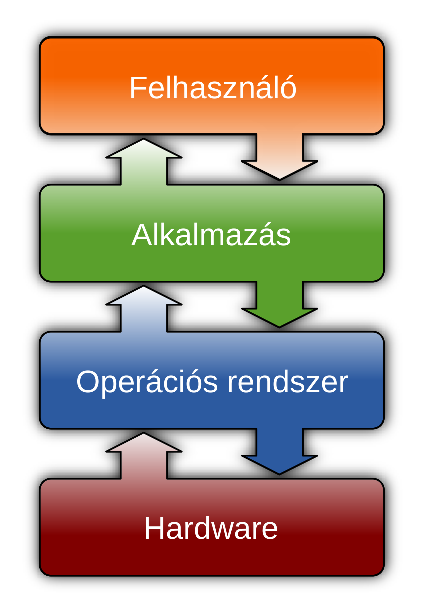
\includegraphics[width=0.8\textwidth]{images/os-hu.eps}
	\end{figure}
\end{columns}
}


\only<5>{
\begin{columns}
	\column{0.45\linewidth}
	\begin{exampleblock}{Booting}
		\begin{itemize}
			\item Manapság a kernel és a hardver között vannak egyebek is
			\item $\sim 2012$ óta az UEFI felváltotta az addigi BIOS alapú bootot
			\item Bonyolult folyamat (POST $\to$ boot loader $\to$ kernel $\to$ OS)
		\end{itemize}
	\end{exampleblock}

	\column{0.5\linewidth}
	\begin{figure}
		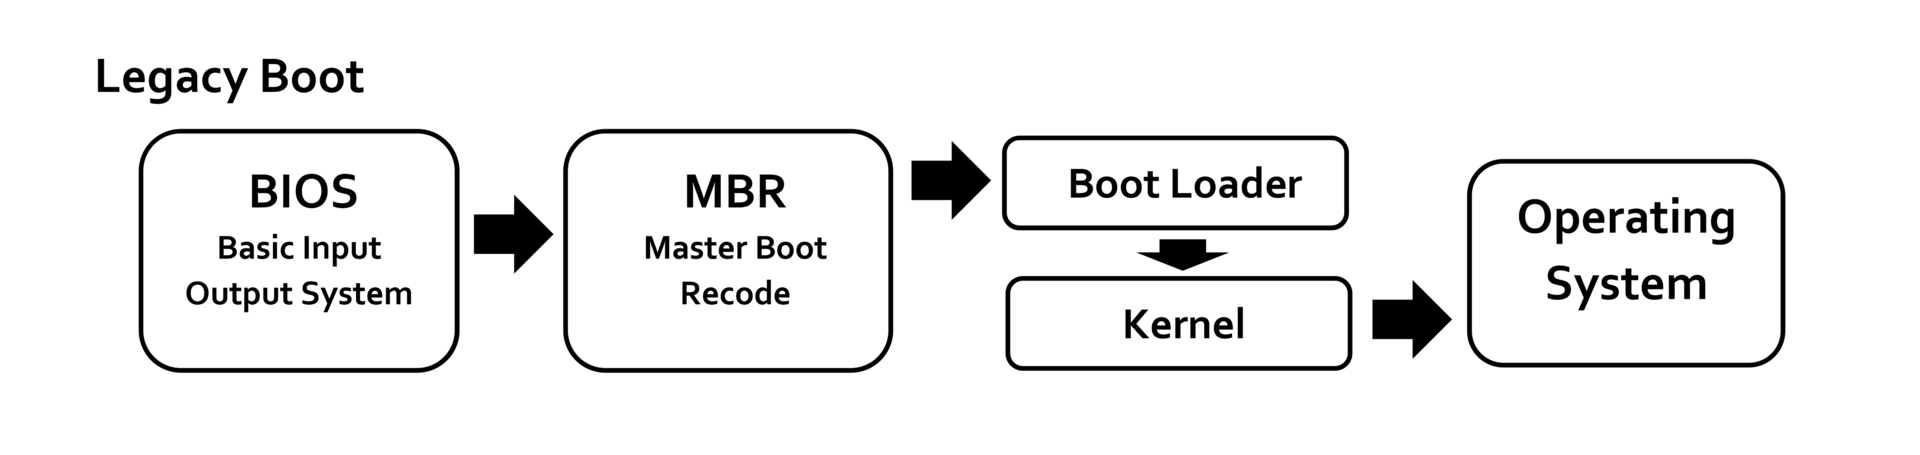
\includegraphics[width=0.9\textwidth]{images/legacy-boot.png}
		\vspace{5pt}
		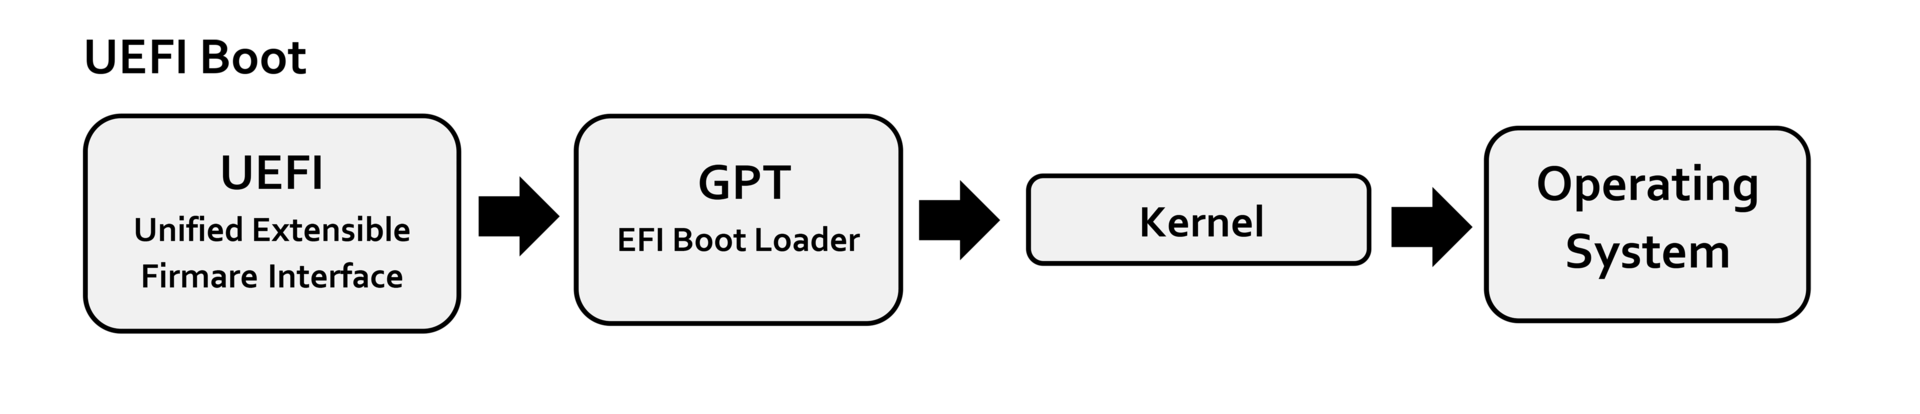
\includegraphics[width=0.9\textwidth]{images/uefi-boot.png}
		\vspace{5pt}
		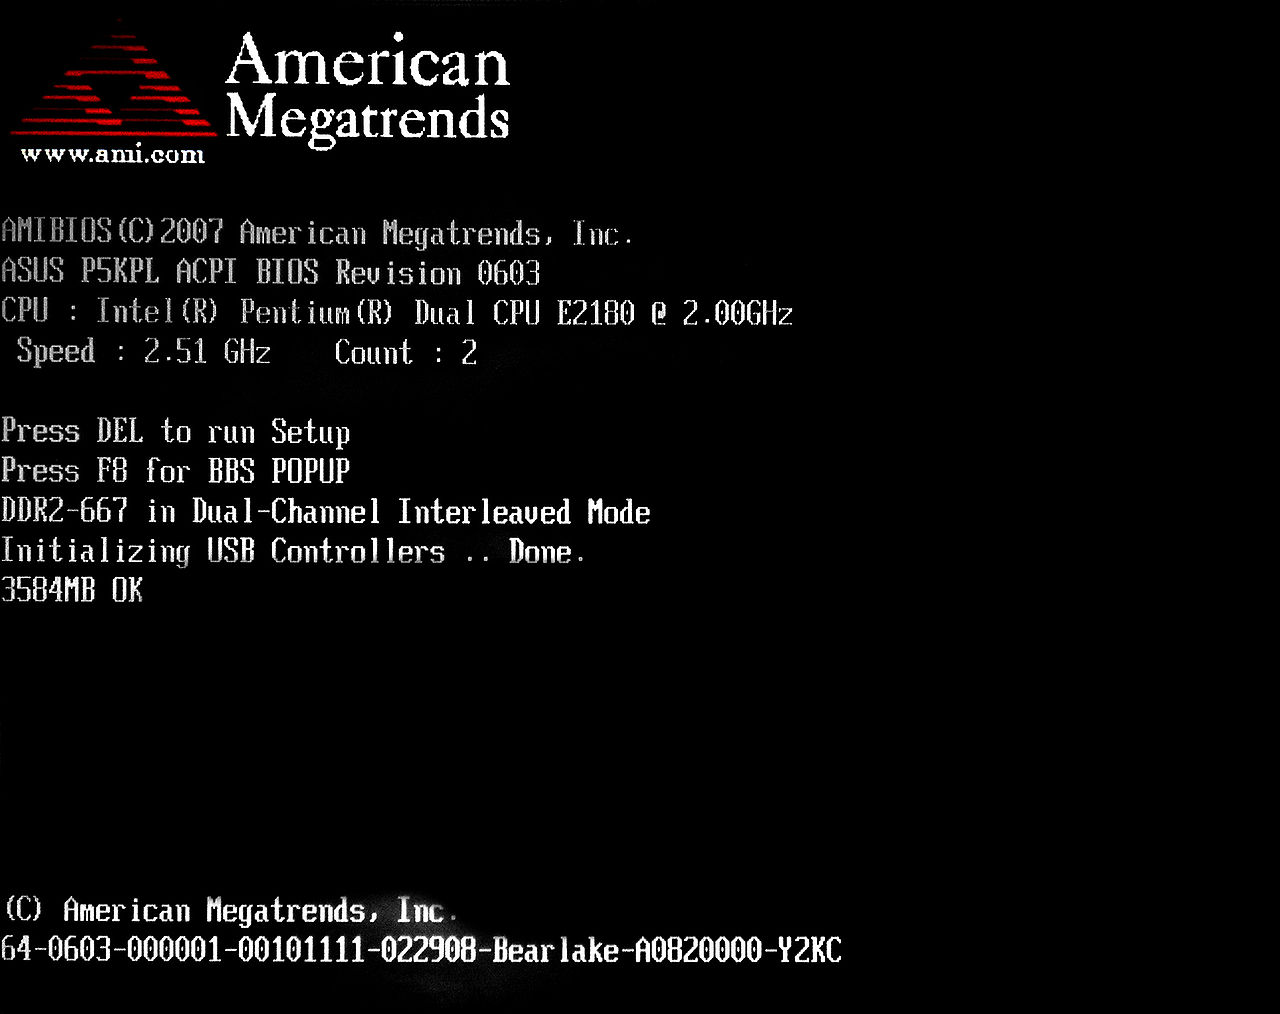
\includegraphics[width=0.9\textwidth]{images/POST.jpg}
	\end{figure}
\end{columns}
}

\end{frame}